\newpage
\section{Prospetto economico}
In questo paragrafo sono presentate, per ciascun periodo del progetto, le ore di impegno calcolate a preventivo per i ruoli coinvolti, divise tra ore di lavoro e ore contabilizzate.\\
 Si ricorda che il periodo di \ARM\ non è a carico del \termine{committente} e quindi non sarà considerata nel calcolo del preventivo.
 
\subsection{\ARD}
Nel periodo riguardante la fase di \ARD\ le ore tra i ruoli sono state divise nel seguente modo:

\begin{table}[h]
	\begin{center}
		\begin{tabular}{|l|c|c|}
			\hline
			\textbf{Ruolo}	& \textbf{Ore} & \textbf{Costo} \\
			\hline
			\textit{\Pm} &	5	&	 150	\\
			\hline
			\textit{\Am}	&	5	&	 100	\\
			\hline
			\textit{\An}	&	18	&	 450	\\
			\hline
			\textit{\Ver}	 & 11	&	 165	\\
			\hline
			\textbf{Totale} &	 39	&	865	\\
			\hline
		\end{tabular}
	\end{center}
	\caption{Incidenza ore su costo per ruolo, \ARD}
\end{table}

\begin{figure}[H]
	\centering 
	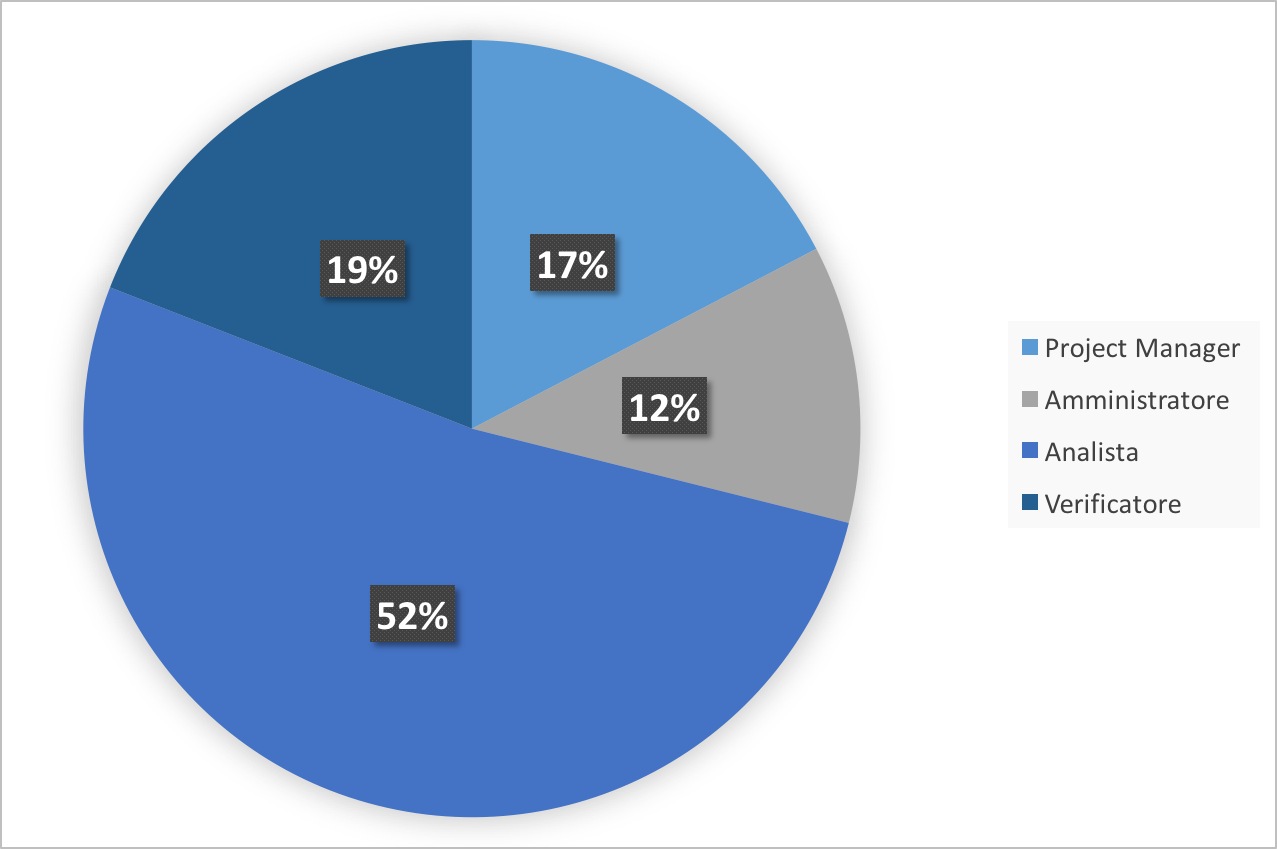
\includegraphics[scale=0.7]{Immagini/GraficiTorteSezione6/ARD.png}
	\caption{Costo per ruolo, \ARD}
\end{figure}

\newpage
\subsection{\PA}
Nel periodo riguardante la \PA\ le ore tra i ruoli sono state divise nel seguente modo:

\begin{table}[h]
	\begin{center}
		\begin{tabular}{|l|c|c|}
			\hline
			\textbf{Ruolo}	& \textbf{Ore} &	\textbf{Costo}	 \\
			\hline
			\textit{\Pm}	&	6	&	180		\\
			\hline
			\textit{\Am}	&	8	&	160		\\
			\hline
			\textit{\Prog}	&	129	&	2838	\\
			\hline
			\textit{\Ver}	&	62	&	930	\\
			\hline
			\textbf{Totale}	&	205	&	4108	\\
			\hline
		\end{tabular}
	\end{center}
	\caption{Incidenza ore su costo per ruolo, \PA}
\end{table}

\begin{figure}[H]
	\centering 
	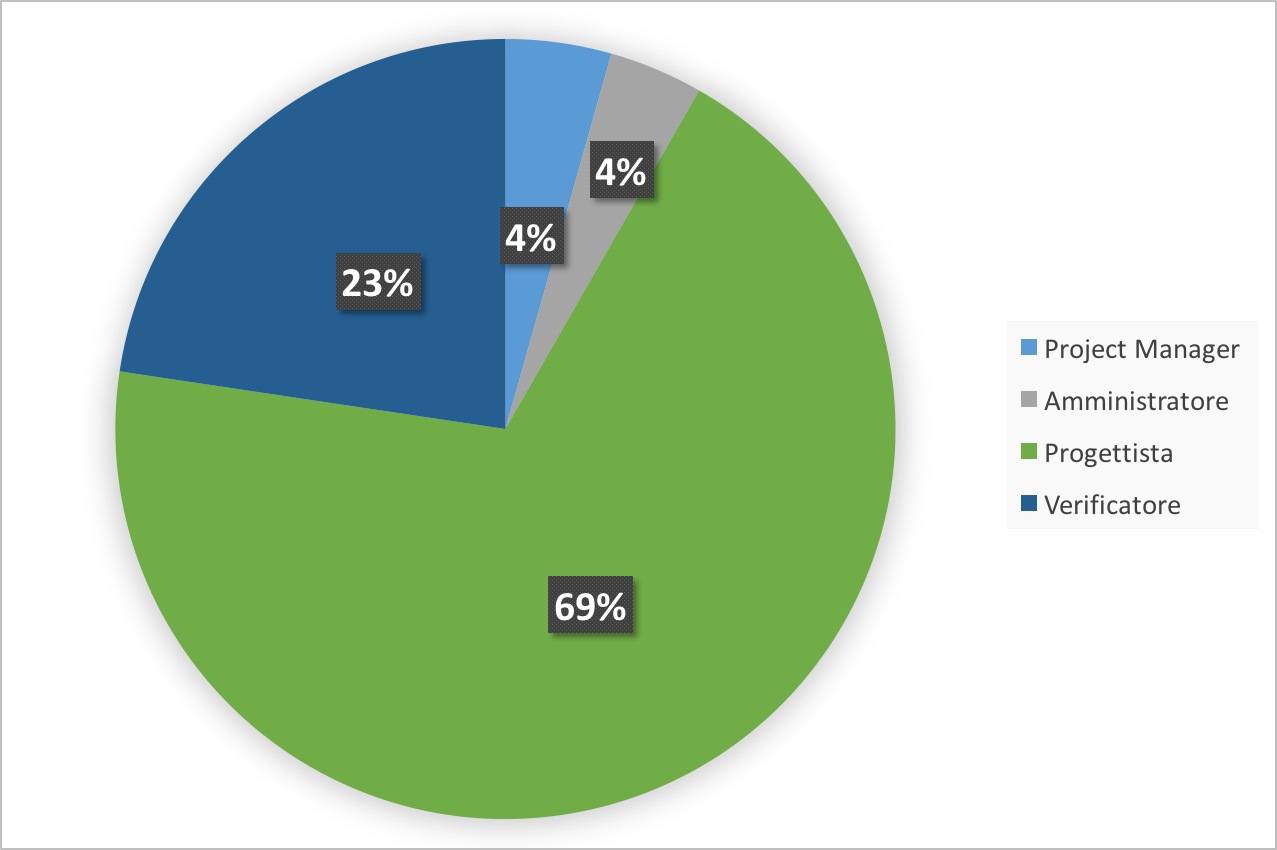
\includegraphics[scale=0.7]{Immagini/GraficiTorteSezione6/PA.png}
	\caption{Costo per ruolo, \PA}
\end{figure}

\newpage
\subsection{\PD}
Nel periodo riguardante la \PD\ le ore tra i ruoli sono state divise nel seguente modo:

\begin{table}[h]
	\begin{center}
		\begin{tabular}{|l|c|c|}
			\hline
			\textbf{Ruolo}	& \textbf{Ore} &	\textbf{Costo}	 \\
			\hline
			\textit{\Pm}	&	7	&	210		\\
			\hline
			\textit{\Am}	&	7	&	140		\\
			\hline
			\textit{\Prog}	&	76	&	1672	\\
			\hline
			\textit{\Ver}	&	38	&	570		\\
			\hline
			\textbf{Totale}	&	128	&	2592	\\
			\hline
		\end{tabular}
	\end{center}
	\caption{Incidenza ore su costo per ruolo, \PD}
\end{table}

\begin{figure}[H]
	\centering 
	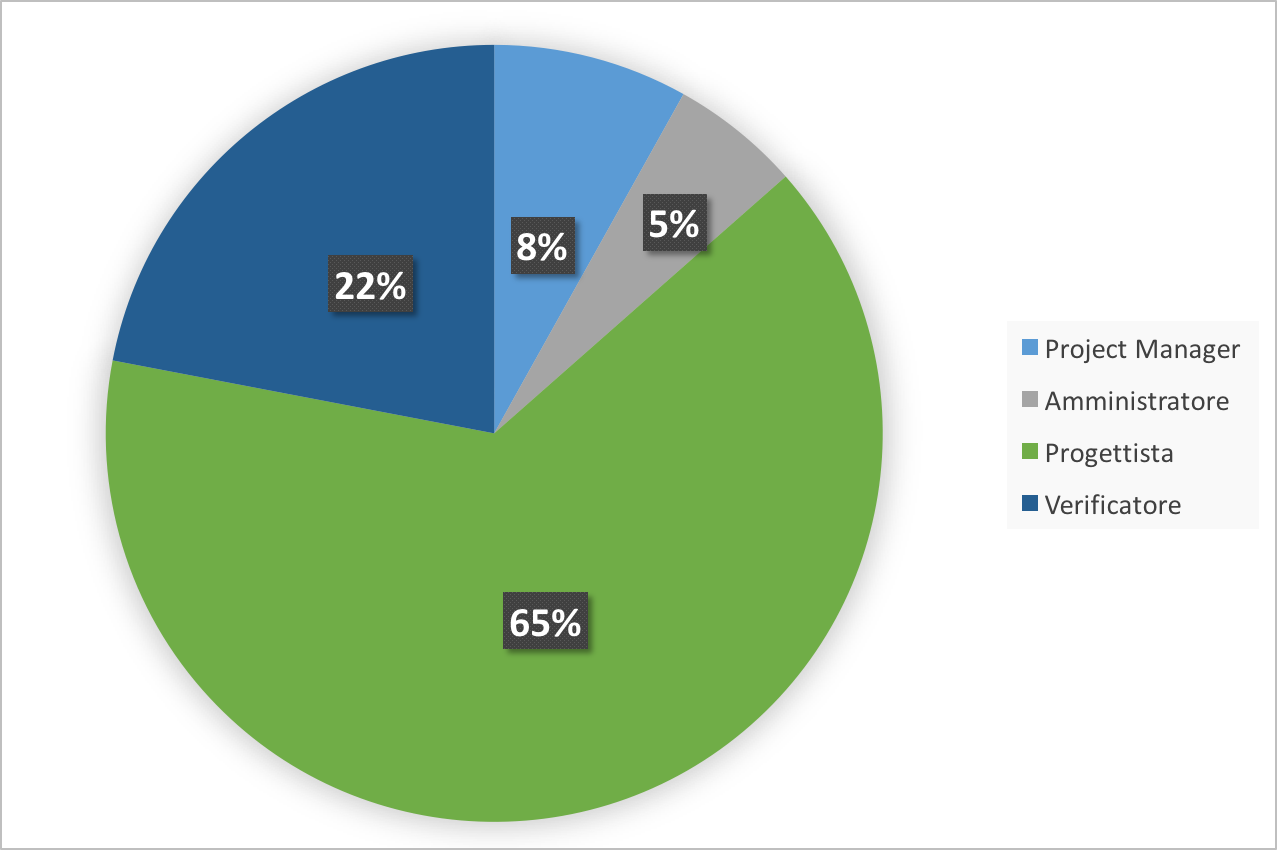
\includegraphics[scale=0.7]{Immagini/GraficiTorteSezione6/PD.png}
	\caption{Costo per ruolo, \PD}
\end{figure}

\newpage
\subsection{\COD}
Nel periodo riguardante la \COD\ le ore tra i ruoli sono state divise nel seguente modo:

\begin{table}[h]
	\begin{center}
		\begin{tabular}{|l|c|c|}
			\hline
			\textbf{Ruolo}	& \textbf{Ore} &	\textbf{Costo}	 \\
			\hline
			\textit{\Pm}	&	11	&	330		\\
			\hline
			\textit{\Am}	&	6	&	120		\\
			\hline
			\textit{\Prog}	&	21	&	462		\\
			\hline
			\textit{\Progr}	&	132	&	1980	\\
			\hline
			\textit{\Ver}	&	60	&	900	\\
			\hline
			\textbf{Totale}	&	230	&	3792	\\
			\hline
		\end{tabular}
	\end{center}
	\caption{Incidenza ore su costo per ruolo, \COD}
\end{table}

\begin{figure}[H]
	\centering 
	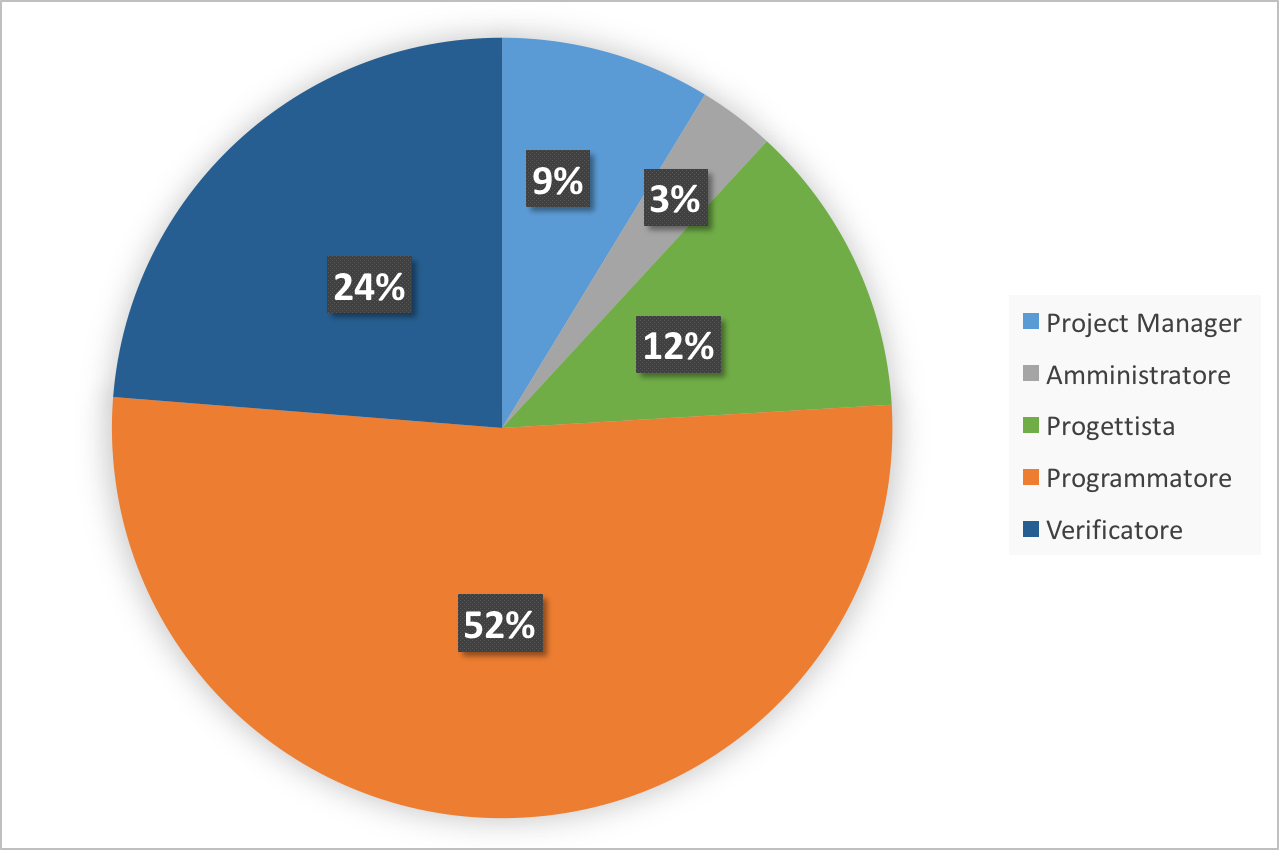
\includegraphics[scale=0.7]{Immagini/GraficiTorteSezione6/COD.png}
	\caption{Costo per ruolo, \COD}
\end{figure}

\newpage
\subsection{\VV}
Nel periodo riguardante la \VV\ le ore tra i ruoli sono state divise nel seguente modo:

\begin{table}[h]
	\begin{center}
		\begin{tabular}{|l|c|c|}
			\hline
			\textbf{Ruolo}	& \textbf{Ore} &	\textbf{Costo}	 \\
			\hline
			\textit{\Pm}	&	12	&	360		\\
			\hline
			\textit{\Am}	&	8	&	160		\\
			\hline
			\textit{\Prog}	&	22	&	484	\\
			\hline
			\textit{\Ver}	&	84	&	1260	\\
			\hline
			\textbf{Totale}	&	126	&	2264	\\
			\hline
		\end{tabular}
	\end{center}
	\caption{Incidenza ore su costo per ruolo, \VV}
\end{table}

\begin{figure}[H]
	\centering 
	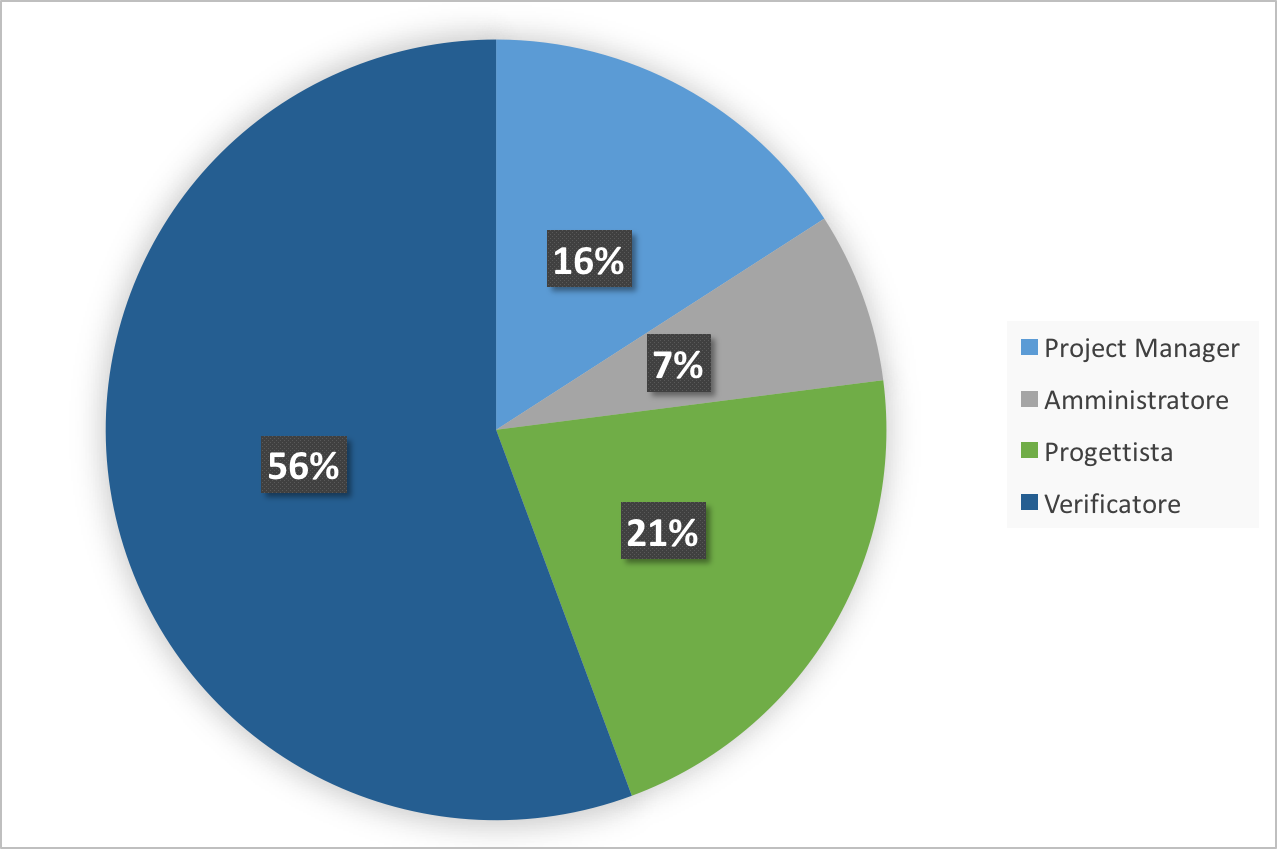
\includegraphics[scale=0.7]{Immagini/GraficiTorteSezione6/VV.png}
	\caption{Costo per ruolo, \VV}
\end{figure}

\newpage
\subsection{Totale}
\subsubsection{Ore totali}
Le ore totali, previste per la realizzazione dell'intero progetto, comprese le ore di investimento, sono riportate nella tabella seguente.

\begin{table}[h]
	\begin{center}
		\begin{tabular}{|l|c|c|c|}
			\hline
			\textbf{Ruolo}	& \textbf{Ore} &	\textbf{Ore remunerabili}	 &\textbf{Costo} \\
			\hline
			\textit{\Pm}	&	67	&	41	&	1230	\\
			\hline
			\textit{\Am}	&	54	&	34	&	680	\\
			\hline
			\textit{\An}	&	91	&	18	&	450	\\
			\hline
			\textit{\Prog}	&	248	&	248	&	5456	\\
			\hline
			\textit{\Progr}	&	132	&	132	&	1980	\\
			\hline
			\textit{\Ver}	&	311	&	255	&	3825	\\
			\hline
			\textbf{Totale}	&	903	&	728	&	13621	\\
			\hline
		\end{tabular}
	\end{center}
	\caption{Costo totale per ruolo}
\end{table}

\begin{figure}[H]
	\centering 
	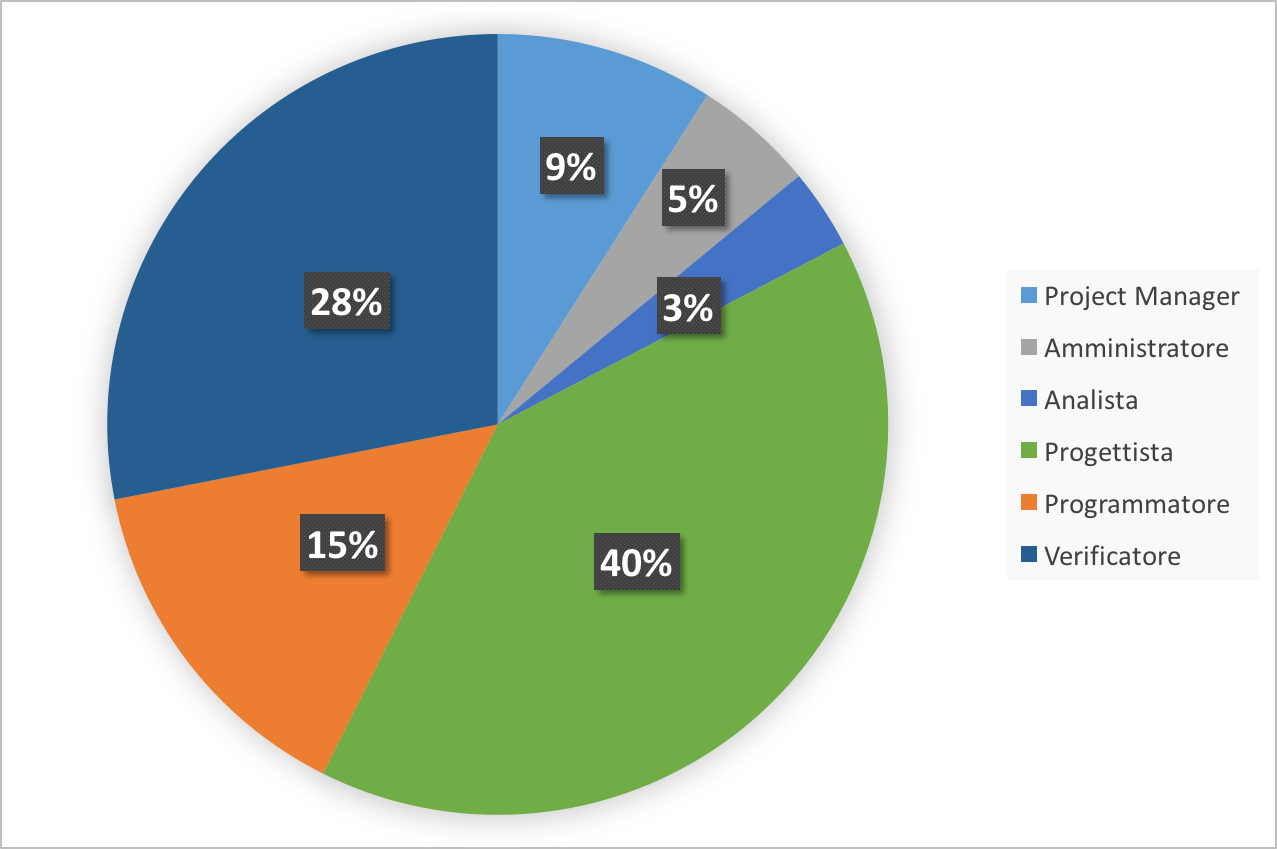
\includegraphics[scale=0.7]{Immagini/GraficiTorteSezione6/TOT.png}
	\caption{Costo totale per ruolo}
\end{figure}

\subsubsection{Conclusioni}
Il costo totale del progetto, indicato nella tabella 20, viene arrotondato a \textbf{\euro 13621}.\\